\documentclass[12pt,a4paper]{article}
\usepackage[margin=1.25in]{geometry}
\usepackage{fancyhdr} % fancy header
\pagestyle{fancy} % so fancy
\usepackage[russian,english]{babel} % for russian letters
\usepackage{tipa} % for IPA symbols
\usepackage[round]{natbib} % bibliography
\usepackage{graphicx} % for importing graphics / figures
\usepackage{booktabs} % publication-worthy tables
\usepackage{adjustbox} % makes tables fit nicely on the page
\usepackage{hyperref}
\usepackage{wrapfig}

\lhead{Joshua MEYER}
\rhead{Google AI Follow-up}
\cfoot{} %% make empty to get rid of the page number %% \cfoot{Page \thepage}
\renewcommand{\footrulewidth}{0.4pt} %% this puts a fancy line at the footer


\begin{document}





\subsubsection*{Research Passion}



\begin{center}
\textit{Everyone should have access to speech technology in their native language.}
\end{center}

This is the conviction that drives my research. I want the world to be a place where someone born blind doesn't have to settle for a lesser education because of lack of audiobooks. Unfortunately, in our current world this is a real problem. I've worked with people in that exact situation to build a free Kyrgyz speech synthesizer. In this way, I've played a small role to make speech technologies accessible, but there is a hard limit as to what I can accomplish on my own.

The Google AI residency is the next step towards my goals. I want to publish influential work and get more people caring about low-resource languages. With my knowledge of linguistics and passion for machine learning, the Google Brain team is the perfect place for me to learn, collaborate, and share my research with others. In particular, I have many ideas for multilingual speech technologies, extracting information from large datasets to transfer knowledge to smaller domains. Working with Google researchers, I am confident I can tackle these problems.

The competitive (yet collaborative) research atmosphere at Google excites me, and I can offer my enthusiasm and dedication to research. 


\subsubsection*{Open-endedness}

My thesis topic is Low-Resource Multi-Task Learning for Deep Neural Network Acoustic Modeling in Automatic Speech Recognition (ASR).

Acoustic models in ASR are classifiers which accept some speech signal (ie. time chunks of audio) and return probabilities over phonetic transcriptions. I use a Multi-Task feedforward neural network (ie. multiple output layers) to perform this classification. Learning related tasks in parallel can improve performance on the main task, because the weights in the net will be biased towards general, task-independent representations of the data (Caruana 1997).

The Multi-Task approach offers an elegant way to exploit small datasets, if you can come up with the right tasks. In my recent experiments, I created auxiliary tasks using linguistic theory, lowering Word Error Rates for small data sets. Where previous Multi-Task work found no improvement using linguistic categories, I improved over my single-task baseline model by reformulating the problem.

Labels in acoustic modeling are isolated speech sounds such as \texttt{[b]} or \texttt{[f]}. In reality, a single speech sound is a bundle of linguistic features, such as vocal chord vibration, tongue placement, lip rounding, air turbulence, etc. Past Multi-Task research in this area created extra tasks by predicting each linguistic dimension in isolation (Stadermann 2005). This is like taking a 3-dimensional label \texttt{[x,y,z]}, and predicting \texttt{[x]} and \texttt{[y]} and \texttt{[z]} as additional tasks. The problem with this approach is that the predictive power of any one dimension is very weak.

Reformulating the problem, I created tasks by \textit{removing} one dimension for each task, projecting into \texttt{N-1}-dimensional spaces. That is, instead of \texttt{[x,y,z]} $\rightarrow$ \texttt{[x]} and \texttt{[y]} and \texttt{[z]}, I projected \texttt{[x,y,z]} $\rightarrow$ \texttt{[x,y]} and \texttt{[y,z]} and \texttt{[x,z]}. This approach improves performance, lowering Word Error Rates. These \texttt{N-1}-dimensional spaces have more predictive power, and also force the net to learn the importance of each dimension.

However, defining each task by hand is not a scalable approach. Since then, I've devoted my research to finding scalable, automatic solutions to task creation.

\subsubsection*{Multi-Task as Ensemble}

A Multi-Task classifier is a special case of an ensemble model, where the feature extractors are trained in parallel. Once I made that connection, I found a mass of inspiration from past ensemble work. Looking for \textit{scalable} ensemble model approaches, I came across the Random Forest.

A Random Forest is created by training multiple trees on random re-samples of the data. Each subsample has its own decision plane, specific to its particular data and noise. By voting among all trees, noise is ignored but data generalities remain. Extending this approach, my current research investigates Multi-Task neural nets, where the tasks are random subsets of the data.


\begin{wrapfigure}{L}{0.375\textwidth}
\centering
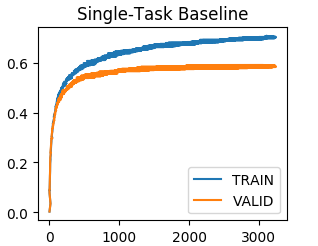
\includegraphics[width=0.35\textwidth]{figs/stl.png}
\end{wrapfigure}

The figure to the left is my current baseline model performance (on Train and Validation) with a 5-layer Time-Delay Neural Network, with 200 dimensional hidden layers. Training data is a 5-hour section of the LibriSpeech corpus. The x-axis is number of iterations, and the y-axis is audio-frame classification accuracy. This model has overfit the training data. Over time, training data accuracy increases, but accuracy on the validation data plateaus and eventually decreases. 


\begin{wrapfigure}{R}{0.4\textwidth}
  \centering
  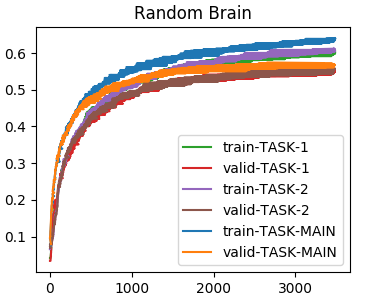
\includegraphics[width=0.35\textwidth]{figs/mtl.png}
\end{wrapfigure}

To the right is the performance of my Multi-Task model (I dub the `Random Brain'). This model is currently training on an Amazon instance with 30 auxiliary tasks (I am only showing 2 auxiliary tasks here). The tasks are random, 50\% subsets of the dataset. The main task is the entire dataset. My impressions from this early data are the following: the Random Brain achieves lower accuracy, but less plateauing compared to the Single-Task model (given the same amount of training iterations). This could mean the extra tasks are a hindrance (making the task harder to learn), or the tasks are harshly penalizing overfitting, and given enough iterations the Random Brain will outperform the baseline on the held-out test data. If this approach works, then the Random Brain could be used to train \textit{any neural net} on \textit{any dataset}. This excites me, because it's potentially a solution which could impact the field of machine learning as a whole, not just speech recognition.


The open-endedness of research does not faze me. I know my goal (make speech technology for all languages), and I know I can happily spend a career chipping away at it. I also know that with Google AI's guidance, I can start chipping better.

\end{document}



 
